\documentclass[12pt]{article}
\usepackage[top=1in,left=1in, right = 1in, footskip=1in]{geometry}

\usepackage{graphicx}
\usepackage{xspace}
%\usepackage{adjustbox}

\newcommand{\comment}{\showcomment}
%% \newcommand{\comment}{\nocomment}

\newcommand{\showcomment}[3]{\textcolor{#1}{\textbf{[#2: }\textsl{#3}\textbf{]}}}
\newcommand{\nocomment}[3]{}

\newcommand{\jd}[1]{\comment{cyan}{JD}{#1}}
\newcommand{\swp}[1]{\comment{magenta}{SWP}{#1}}
\newcommand{\bmb}[1]{\comment{blue}{BMB}{#1}}
\newcommand{\djde}[1]{\comment{red}{DJDE}{#1}}

\newcommand{\eref}[1]{Eq.~\ref{eq:#1}}
\newcommand{\fref}[1]{Fig.~\ref{fig:#1}}
\newcommand{\Fref}[1]{Fig.~\ref{fig:#1}}
\newcommand{\sref}[1]{Sec.~\ref{#1}}
\newcommand{\frange}[2]{Fig.~\ref{fig:#1}--\ref{fig:#2}}
\newcommand{\tref}[1]{Table~\ref{tab:#1}}
\newcommand{\tlab}[1]{\label{tab:#1}}
\newcommand{\seminar}{SE\mbox{$^m$}I\mbox{$^n$}R}

\usepackage{amsthm}
\usepackage{amsmath}
\usepackage{amssymb}
\usepackage{amsfonts}

\usepackage{lineno}
\linenumbers

\usepackage[pdfencoding=auto, psdextra]{hyperref}

\usepackage{natbib}
\bibliographystyle{chicago}
\date{\today}

\usepackage{xspace}
\newcommand*{\ie}{i.e.\@\xspace}

\usepackage{color}

\newcommand{\Rx}[1]{\ensuremath{{\mathcal R}_{#1}}\xspace} 
\newcommand{\Ro}{\Rx{0}}
\newcommand{\Rc}{\Rx{\mathrm{c}}}
\newcommand{\Ri}{\Rx{\mathrm{i}}}
\newcommand{\RR}{\ensuremath{{\mathcal R}}\xspace}
\newcommand{\Rhat}{\ensuremath{{\hat\RR}}}
\newcommand{\Rnaive}{\ensuremath{{\mathcal R}_{\textrm{\tiny naive}}}\xspace}
\newcommand{\tsub}[2]{#1_{{\textrm{\tiny #2}}}}
\newcommand{\dd}[1]{\ensuremath{\, \mathrm{d}#1}}
\newcommand{\dtau}{\dd{\tau}}
\newcommand{\dx}{\dd{x}}
\newcommand{\dsigma}{\dd{\sigma}}

\newcommand{\tstart}{\ensuremath{\tsub{t}{start}}\xspace}
\newcommand{\tend}{\ensuremath{\tsub{t}{end}}\xspace}

\newcommand{\betaeff}{\ensuremath{\tsub{\beta}{eff}}\xspace}
\newcommand{\Keff}{\ensuremath{\tsub{K}{eff}}\xspace}

\newcommand{\pt}{p} %% primary time
\newcommand{\st}{s} %% secondary time

\newcommand{\psize}{{\mathcal P}} %% primary cohort size
\newcommand{\ssize}{{\mathcal S}} %% secondary cohort size

\newcommand{\gtime}{\sigma} %% generation interval
\newcommand{\gdist}{g} %% generation-interval distribution

\newcommand{\geff}{g_{\textrm{eff}}} %% generation-interval distribution

\newcommand{\total}{{\mathcal T}} %% total number of serial intervals

\newcommand{\PP}{{\mathcal P}}
\newcommand{\II}{{\mathcal I}}

\begin{document}

\begin{flushleft}{
	\Large
	\textbf\newline{
		Quantifying the effects of strength- and speed-like responses on epidemic dynamics
	}
}
\newline
\\
Sang Woo Park\textsuperscript{1,*}, Kaiyuan Sun, Benjamin M. Bolker, Bryan T. Grenfell, Jonathan Dushoff, \swp{and maybe others if needed?}
\\
\bigskip
\textbf{1} Department of Ecology and Evolutionary Biology, Princeton University, Princeton, NJ, USA
\\
\bigskip

*Corresponding author: swp2@princeton.edu
\end{flushleft}

\section{Introduction}

The reproduction number \RR---typically defined as the average number of new infections caused by an infected individual---is a key characteristic of an emerging epidemic.
Its value in a fully susceptible population---the \emph{basic} reproduction number, \Ro---provides information about whether a pathogen can invade, the level of intervention required to prevent invasion, and the final size of an epidemic \citep{diekmann1990definition,anderson1991infectious}.
When an epidemic is ongoing, transmission dynamics are affected by changes in population-level immunity, non-pharmaceutical interventions, and contact patterns---
these changes in transmission dynamics can be described by $\RR(t)$, often referred to as the \emph{effective} or \emph{time-dependent} reproduction number \citep{wallinga2004different, fraser2007estimating, cori2013new}.
Interpretation and estimation of $\RR(t)$ have been a key area of research during the ongoing COVID-19 pandemic due to its policy implications \citep{pan2020association,flaxman2020estimating,gostic2020practical}.

One of the main challenges in interpretating $\RR(t)$ can be attributed, in part, to its standard definition: the average number of new infections caused by an infected individual.
While this definition is biologically intuitive, it is mathematically imprecise as time-dependent reproduction numbers can be defined in multiple ways, depending on the cohort (e.g., a group of individuals who developed symptoms or were infected at the same time) and the types of transmission scenarios (i.e., realized or counterfactual transmission processes).
Here, we primarily focus on two main measures of transmission that look at a cohort of infectees or infectors that were infected at the same time: the instantaneous reproduction number $\Ri(t)$ and the case reproduction number $\Rc(t)$.

First, the instantaneous reproduction number $\Ri(t)$---popularized by \cite{cori2013new}---corresponds to the average number of new infections that an individual infected at time $t$ (i.e., an individual from a cohort of infectees) will generate over the course of their infection if conditions at time $t$ remain unchanged \citep{fraser2007estimating}.
The instantaneous reproduction number $\Ri(t)$ characterizes conditions at time $t$ and provides a real-time estimate of whether the disease will continue to spread if conditions were to stay the same.
However, since transmission dynamics change throughout an epidemic, $\Ri(t)$ is a counterfactual measure and must be interpreted with care.

On the other hand, the case reproduction number $\Rc(t)$---popularized by \cite{wallinga2004different}---corresponds to the average number of new infections that an individual infected at time $t$ generated over the course of their infection.
$\Rc(t)$ is a realized measure, which depends on conditions after time $t$ and can only be estimated retrospectively.
Although the verbal definition for $\RR(t)$ (``the average number of new infections caused by an infected individual'') closely resembles that of $\Rc(t)$, its mathematical definition actually corresponds to that of $\Ri(t)$ \citep{gostic2020practical}.
Due to the imprecision of the verbal definition of $\RR(t)$, the counterfactual quality of $\Ri(t)$ (and therefore, $\RR(t)$) is often neglected in its interpretation---
specifically, in contrast to a widely accepted view, $\Ri(t) > 1$ or $<1$ does not provide information about whether the number of infections is increasing or decreasing at time $t$.

Estimating $\Ri(t)$ and $\Rc(t)$ adds another layer of complexity as it requires knowledge of true incidence of infection $i(t)$ and the generation-interval distribution $g(\tau)$, where generation intervals describe time between infections of an infector and an infectee \citep{svensson2007note}.
Here, we focus on the latter: which generation-interval distributions do we need to correctly estimate $\Ri(t)$ and $\Rc(t)$?
Current frameworks for estimating of $\Ri(t)$ and $\Rc(t)$, including widely-used software such as EpiEstim, rely on a time-independent distribution to estimate $\Ri(t)$ throughout the entire epidemic \citep{cori2013new}.
\cite{gostic2020practical} recently suggested that the intrinsic generation-interval distribution (measuring the intrinsic infectiousness of an infected individual, \cite{champredon2015intrinsic}), which is different from the realized generation-interval distributions, is required to estimate $\Ri(t)$.
However, it was noted more than a decade ago that the required distribution to estimate $\Ri(t)$ can change due to interventions that reduce infectiousness in later stages of infection \citep{fraser2007estimating}.

To answer this question, we provide a mathematical framework that correctly links $\Ri(t)$ and $\Rc(t)$ with the renewal process of infection.
We show that a counterfactual distribution---which we referred to as the instantaneous generation-interval distribution---is required to accurately estimate a counterfactual measure of transmission, $\Ri(t)$.
Likewise, a realized distribution---the backward generation-interval distribution---is required to estimate a realized measure of transmission, $\Rc(t)$;
since the renewal process can be equivalently expressed in terms of both $\Ri(t)$ and $\Rc(t)$ (and their corresponding distributions), we can also estimate $\Rc(t)$ using the instantaneous generation-interval distribution, obtaining a Wallinga-Teunis-like estimator \citep{wallinga2004different}.
Under strength-like interventions (e.g., vaccination, social distancing, and mask wearing)---which we define as interventions whose relative effectiveness depends on population-level coverage (i.e., strength of intervention) but not on time since infection---the instantaneous generation-interval distribution remains unchanged (and therefore is equivalent to the intrinsic distribution).
On the other hand, under speed-like interventions (e.g., self-isolation and contact tracing)---which we define as interventions whose relative effectiveness depends on time since infection (and therefore the speed of intervention)---the instantaneous generation-interval distribution changes.
Neglecting such changes can bias estimates of reproduction numbers (both $\Ri(t)$ and $\Rc(t)$), including when it crosses the threshold of 1.
Instead, we generalize the idea of exponential growth rate $r$ beyond the exponential phase and show that growth rates $r(t)$ are robust under both strength- and speed-like responses as it does not require assumptions about the underlying distribution.

\section{Mathematical theory}

\subsection{Renewal equation framework}

The renewal equation framework provides a flexible way of modeling the spread of infection and the impact of intervention on the spread \citep{fraser2007estimating}.
Let $K(t, \tau)$ represent the infection kernel, defined as the rate at which secondary cases are generated at time $t$ by an individual infected $\tau$ time units ago (we will use $s, t$ to denote calendar time and $\sigma, \tau$ to denote time since infection throughout).
The shape of this kernel can depend on intrinsic factors (e.g., variation in infectiousness over the course of infection) or extrinsic factors (e.g., susceptible depletion, non-pharmaceutical interventions, and changes in behavior).
Then, incidence of infection at time $t$ caused by a cohort of individuals infected $\tau$ time units ago can be written as the product of kernel, $K(t, \tau)$, and incidence at time $t-\tau$, $i(t-\tau)$:
\begin{equation}
i_{t-\tau}(t) = K(t, \tau) i(t-\tau).
\end{equation}
Integrating across time since infection $\tau$ allows us to express the dynamics of the proportion susceptible $S(t)$ and incidence $i(t)$ in the absence of natural births or deaths as follows: 
\begin{align}
\frac{\mathrm{d}S}{\mathrm{d}t} &= - i(t),\\
i(t) &= \int_0^\infty K(t, \sigma) i(t-\sigma) \dsigma.
\label{eq:renewal}
\end{align}
This model, also known as renewal equations, generalizes the dynamics of many compartmental models, including the standard SEIR model \citep{heesterbeek1996concept, diekmann2000mathematical, roberts2004modelling, aldis2005integral, roberts2007model, champredon2018equivalence}.

Here, we show that the same renewal process of infection can be equivalently expressed in terms of instantaneous (counterfactual) quantities as well as realized quantities, meaning $\Ri(t)$ and $\Rc(t)$ with their corresponding generation-interval distributions.
The integral of $K(t, \tau)$ corresponds to the instantaneous reproduction number \citep{fraser2007estimating}: $\Ri(t) = \int K(t, \sigma) \dsigma$.
The kernel, normalized by the total infectiousness, provides information about the time scale of transmission.
We refer to this quantity as the instantaneous generation-interval distribution: $g(t, \tau) = K(t, \tau)/\Ri(t)$.
Both the instantaneous reproduction number and the generation-interval distribution are counterfactual quantities---that is, they describe what their corresponding realized values will be if conditions at time $t$ remain constant (i.e., if $K(s, \tau) = K(t, \tau)$ for all $s \geq t$).
In this case, the renewal equations (\eref{renewal}) can be written as:
\begin{align}
\frac{\mathrm{d}S}{\mathrm{d}t} &= - i(t),\\
i(t) &= \Ri(t) \int_0^\infty g(t, \sigma) i(t-\sigma) \dsigma.
\label{eq:renewal_instantaneous}
\end{align}
For example, in the absence of intervention, we have $\Ri(t) = \Ro S(t)$ and $g(t, \tau) = g_0(\tau)$, where $\Ro$ represents the basic reproduction number and $g_0(\tau)$ represents the intrinsic generation-interval distribution.

Now, consider the forward kernel $F_t(\tau)$, which represents the rate at which an individual infected at time $t$ generates a secondary cases $\tau$ time units after infection: 
\begin{equation}
F_t(\tau) = K(t+\tau, \tau) = \Ri(t + \tau) g(t+\tau, \tau).
\label{eq:fkernel}
\end{equation}
The integral of $F(t, \tau)$, representing the total infectiousness of an individual infected at time $t$, corresponds to the case reproduction number: $\Rc(t) = \int F_t(\sigma) \dsigma$. 
The forward kernel, normalized by the total infectiousness, correspond to the forward generation-interval distribution $f_t(\tau) = F_t(\tau)/\Rc(t)$, describing realized generation intervals for a cohort of infector that were infected at time $t$.
Then, the forward renewal equation can be written as:
\begin{align}
\frac{\mathrm{d}S}{\mathrm{d}t} &= - i(t),\\
i(t) &= \int_0^\infty \Rc(t-\sigma) f_{t-\sigma}(\sigma) i(t-\sigma) \dsigma.
\label{eq:renewal_forward}
\end{align}
The forward renewal equation reveals an important insight: Even if the instantaneous generation-interval distribution $g(t, \tau)$ remains invariant across time (i.e., $g(t, \tau) = g_0(\tau)$), changes in $\Ri(t)$ causes the forward generation-interval distribution to change (see \eref{fkernel}).
Therefore, renewal equation models that rely on the forward form (\eref{renewal_forward}) but assume time-invariant $f_t(\tau)$ are theoretically unjustified and should not be used.

The forward renewal equation further allows us to verify that the instantaneous quantities ($\Ri(t, \tau)$ and $g(t, \tau)$) indeed represent counterfactual conditions:
Assuming that conditions at time $t$ remain constant (i.e., if $K(s, \tau) = K(t, \tau)$ for all $s \geq t$), we obtain $F_{t}(\tau) = K(t, \tau)$ (and therefore, $\Rc(t) = \Ri(t)$ and $f_{t}(\tau) = g(t,\tau)$).
In other words, $\Ri(t)$ and $g(t,\tau)$ describe number of secondary infections that an individual infected at time $t$ will generate, and when these infections will occur, if conditions at time $t$ remain constant;
since transmission dynamics can change rapidly during an ongoing epidemic, instantaneous quantities must be interpreted with care.

\subsection{Strength- and speed-like interventions}

\begin{figure}[!th]
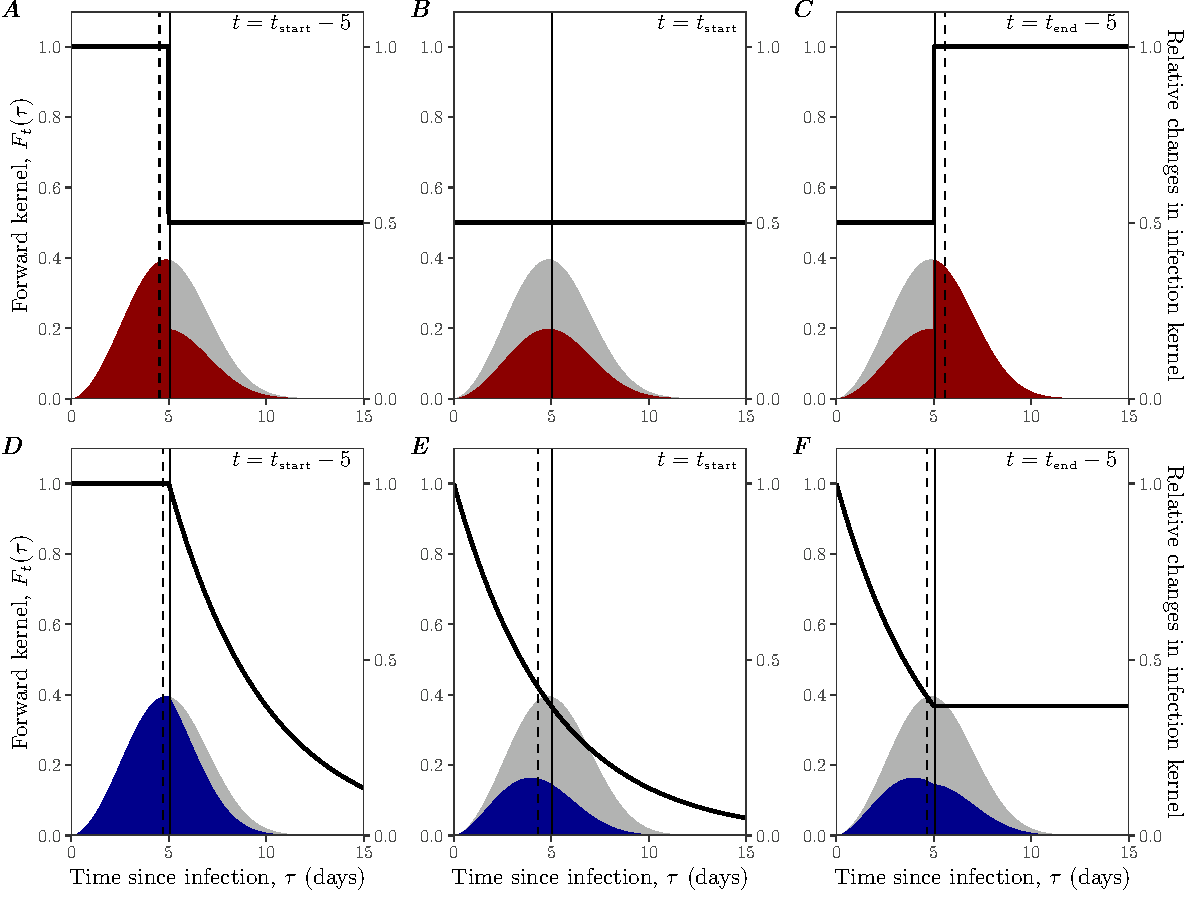
\includegraphics[width=1\textwidth]{pop_ind_compare.pdf}
\caption{
\textbf{The impact of population- and individual-based interventions on forward kernels.}
The impact of constant strength (A--c) and speed (D--F) intervention on forward kernels of individuals infected at different time:
5 days before intervention onset (A, D), during intervention (B, E), and 5 days before intervention offset (C, F).
Gray shaded curves represent the intrinsic kernel $K_0(\tau)$.
Colored curves represent the forward kernel $F_t(\tau)$.
Solid black lines represent relative changes in the kernel: $F_t(\tau)/K_0(\tau)$.
Solid vertical lines the mean intrinsic generation interval.
Dashed vertical lines the mean forward generation interval.
}
\label{fig:indpop}
\end{figure}

To model the impact of intervention during an ongoing epidemic, we first distinguish strength-like interventions, which reduces the infectiousness of all (or some fraction of) infected individuals by a constant amount regardless of their time since infection, from speed-like interventions, which target each infected individual separately and therefore depend on their time of infection \citep{dushoff2021speed}.
Strength-like interventions can be thought of as population-level interventions that reduce the transmission rate and include social distancing, school closures, and vaccination.
Speed-like interventions can be thought of as individual-level interventions that reduce the duration of infectious periods and include case isolation and behavioral changes (e.g., symptomatic individuals are more likely to self-isolate earlier as awareness increases).
While our primary focuses are instantaneous quantities ($\Ri(t)$ and $g(t, \tau)$), we first illustrate the impact of strength- and speed-like interventions using realized (forward) quantities as they describe realized transmission processes and are easier to interpret.

Let $\PP(t)$ represent a strength-like intervention that modulates the infection kernel multiplicatively at calendar time $t$ such that $\PP(t)=1$ corresponds to intervention that has no effect and $\PP(t) < 1$ corresponds to intervention that reduces transmission.
Then, the infection kernel under $\PP$ at calendar time $t$ can be written as:
\begin{equation}
K(t, \tau) = \Ro S(t) \PP(t) g_0(\tau).
\end{equation}
Likewise, the forward kernel of an individual infected at time $t$ under $\PP$ can be written as:
\begin{equation}
F_t(\tau) =  \Ro S(t+\tau) \PP(t + \tau) g_0(\tau).
\end{equation}
Here, we see that strength-like interventions have qualitatively same impact on transmission dynamics as susceptible depletion.

For example, a social distancing measure that reduces transmission rate by a factor of $1/\phi$ (i.e., constant strength) between time \tstart and \tend can be modeled as:
\begin{equation}
\PP(t) = \begin{cases}
1 & t < \tstart\\
\phi & \tstart \leq t < \tend\\
1 & \tend \leq t
\end{cases}.
\end{equation}
\fref{indpop}A--C illustrates the impact of such intervention on the forward kernel of an individual infected 5 days before $\tstart$, at $\tstart$, and 5 days before $\tend$ (assuming $S(t) \approx 1$).
Strength-like interventions can take effect immediately and sharply reduce transmission (\fref{indpop}A);
likewise, lifting the intervention can, in theory, can cause the forward kernel to return back to normal immediately (\fref{indpop}C).
Even though the exact shape of the kernel depends on the time of infection and when the intervention was introduced relative to the infection time, the relative impact of intervention in reducing transmission at any given time (by a factor of $1/\phi$) does not vary across individuals (\fref{indpop}A--C).
Such intervention also has direct effects on realized generation intervals:
implementing (lifting) intervention decreases (increases) future transmission potential and therefore decreases (increases) the mean realized generation interval (\fref{indpop}A,C).
If an individual is infected after \tstart (and much earlier than \tend), this intervention simply reduces the entire kernel by a constant amount and has no effect on realized generation intervals (\fref{indpop}B).
This mechanism explains and further generalizes how susceptible depletion leads to contraction of realized generation intervals in a homogeneously mixing population \citep{kenah2008generation,nishiura2010time,champredon2015intrinsic}. 

On the other hand, a speed-like intervention $\II(t, \tau)$, such as case isolation, targets each infected individual and therefore depends on calendar time $t$ as well as time since infection $\tau$.
In theory, $\II(t, \tau)$ can capture almost all interventions, including strength-like interventions; here, we use $\II(t, \tau)$ to specifically model interventions that take the following form:
\begin{equation}
\II(t, \tau) = \exp \left(- \int_0^\tau h(t-\tau+\sigma, \sigma) \dsigma \right),
\end{equation}
where $h(t, \tau)$ represents the rate at which an individual infected $\tau$ time units ago will be isolated at calendar time $t$.
Then, $\II(t,\tau)$ can be interpreted as the probability that an individual infected $\tau$ time units ago has not been isolated by calendar time $t$.
In this case, the infection kernel under $\II$ at calendar time $t$ is given by:
\begin{equation}
K(t, \tau) = \Ro S(t) \II(t, \tau) g_0(\tau).
\end{equation}
Likewise, the forward kernel of an individual infected at time $t$ under $\II$ can be written as:
\begin{equation}
F_t(\tau) = \Ro S(t+\tau) \II(t+\tau, \tau) g_0(\tau).
\end{equation}
This intervention is speed-like because its effectiveness depends on how fast we can isolate infected individuals.

For example, given hazard $h(\tau)$ of being isolated, the probability that an individual infected at time $t$ has not been isolated by $\tau$ time units after infection given that the intervention takes place between time \tstart and \tend depends on the amount of time the individual has been exposed to this intervention.
If the individual is infected before $\tstart$, they will not be isolated by this intervention until after $\tstart$.
If the individual is infected after $\tend$, they will never be isolated by this intervention.
Therefore, such intervention can be modeled as:
\begin{equation}
\II(t+\tau, \tau) = \begin{cases}
1 & t < \tstart-\tau \\
\exp\left(- \int_{\max(0, \tstart - t)}^{\min(\tau, \tend-t)} h(\sigma)\dd{\sigma} \right) & \tstart-\tau \leq t < \tend \\
1 & \tend \leq t
\end{cases}
\end{equation}
\fref{indpop}D--E illustrates the impact of a speed-like intervention with constant hazard on the forward kernel of an individual infected 5 days before $\tstart$, at $\tstart$, and 5 days before $\tend$ (assuming $S(t) \approx 1$).
Unlike the strength-like intervention, speed-like intervention does not take effect immediately;
that is, the rate at which an infected individual generates secondary infections at time $\tstart$ (e.g., $F_t(\tstart-t)$ in \fref{indpop}D; more generally, $K(\tstart, \tau)$) remains unaffected by the intervention because it takes time to identify and isolate infected individuals.
On the other hand, when the intervention is lifted at $\tend$, the value of the kernel at calendar time $\tend$ ($F_t(\tend-t)$ in \fref{indpop}F; more generally, $K(\tend, \tau)$) remains unchanged because some fraction of infected individuals have already been isolated.
In general, speed-like interventions shorten realized generation intervals because they prevent late transmission (\fref{indpop}D--E).

Finally, given strength- and speed-like interventions, $P(t)$ and $I(t, \tau)$, the infection kernel can be written as:
\begin{equation}
K(t, \tau) = \Ro S(t) \PP(t) \II(t,\tau) g_0(\tau).
\end{equation}
The corresponding forward kernel can be written as:
\begin{equation}
F_t(\tau) = \Ro S(t+\tau) \PP(t + \tau) \II(t+\tau, \tau) g_0(\tau).
\end{equation}
Therefore, the dynamics of $S(t)$ and $i(t)$ can be now written as:
\begin{align}
\frac{\mathrm{d}S}{\mathrm{d}t} &= - i(t),\\
i(t) &= \Ro S(t) \PP(t) \int_0^\infty \II(t, \sigma) g_0(\sigma) i(t-\sigma)\dsigma.
\end{align}
In this case, the instantaneous reproduction number and generation-interval distributions are given by:
\begin{align}
\Ri(t) &= \RR_0 S(t) \PP(t) \int_0^\infty \II(t,\sigma) g_0(\sigma) \dsigma,\\
g(t, \tau) &= \frac{\II(t,\tau) g_0(\tau)}{\int_0^\infty \II(t,\sigma) g_0(\sigma) \dsigma},
\end{align}
which allow us to express the renewal equation in the form of \eref{renewal_instantaneous}.
Therefore, the instantaneous generation-interval distribution changes under speed-like interventions but not under strength-like interventions, even though both types of interventions affect the realized generation-interval distribution.

% probably belongs in the discussion
% Current frameworks for estimating $\Ri(t)$ assume that all interventions are strength-like and neglect the possibility that they might be speed-like.
% While many non-pharmaceutial interventions that were implemented during the current COVID-19 pandemic are strength-like (e.g., social distancing, school closures, limiting the size of gatherings, and vaccination), they can still elicit speed-like behavioral changes as infected individuals can become more likely to self-isolate faster after they have developed symptoms.

\subsection{Quantifying changes in instantaneous generation-interval distributions}

In order to accurately model the renewal process, we have to be able to first quantify how the instantaneous generation-interval distribution $g(t, \tau)$ changes across time $t$.
The instantaneous distribution measures the infectiousness of an individual infected $\tau$ time units ago at time $t$ and is therefore different from the distribution of realized generation intervals (i.e., time between actual infection events).
For example, if we were to take all realized generation intervals that end at time $t$ and form a distribution, we obtain what is known as the backward generation-interval distribution, $b_t(\tau)$:
\begin{align}
b_t(\tau) &= \frac{i_{t-\tau}(t)}{\int_0^\infty i_{t-\sigma}(t) \dsigma},\label{eq:backward}\\
&= \frac{g(t,\tau) i(t-\tau)}{\int_0^\infty g(t,\sigma) i(t-\sigma) \dsigma},\label{eq:b1}\\
&= \frac{\Rc(t-\tau) f_{t-\tau}(\tau) i(t-\tau)}{\int_0^\infty \Rc(t-\sigma) f_{t-\sigma}(\sigma) i(t-\sigma) \dsigma},\label{eq:b2}
\end{align}
which depends on previous incidence of infection (\eref{b1}) as well as the case reproduction $\Rc$ of previously infected individuals (\eref{b2}), depending on the generation-interval distribution we try to link with.
Several studies have noted, in many contexts, that backward distributions provide biased estimates of the forward distribution due to such dependence \citep{nishiura2010time,champredon2015intrinsic,park2020inferring,park2020forward}.

The forward distributions are also different from the instantaneous distributions.
While both the forward generation-interval distribution $f_{t-\tau}(\tau)$ and the instantaneous generation-interval distribution $g(t, \tau)$ depend on the rate at which secondary cases at time $t$ are generated by a primary case infected at time $t-\tau$, $K(t, \tau)$, they are normalized by different quantities:
\begin{equation}
f_{t-\tau}(\tau) = \frac{K(t,\tau)}{\int_0^\infty K(t-\tau+\sigma,\sigma) \dsigma} \neq \frac{K(t,\tau)}{\int_0^\infty K(t,\sigma) \dsigma} = g(t, \tau).
\end{equation}
The forward distribution $f_{t-\tau}(\tau)$ is normalized by the average number of new infections caused by an individual infected at time $t-\tau$ (i.e., the case reproduction number, $\Rc(t-\tau)$).
On the other hand, the instantaneous distribution $g(t, \tau)$ is normalized by the sum of average number of new infections that an individual infected at time $t-\sigma$ generated at time $t$ (integrated across $\sigma$).

Therefore, even if we can observe all realized generation intervals throughout an epidemic, estimating the instantaneous distribution $g(t, \tau)$ is not trivial.
Even within a homogeneously mixing population, in which the disease is allowed to spread unchecked (and therefore $g(t, \tau) = g_0(\tau)$ for all $t$), aggregating all realized generation intervals underestimates the mean intrinsic generation interval due to susceptible depletion \citep{park2020inferring}.
Either a deconvolution or a novel statistical tool is needed to accurately estimate the instantaneous distribution $g(t, \tau)$.
To our knowledge, no studies have accomplished this yet.

\subsection{Quantifying changes in time-dependent reproduction numbers}

The impact of intervention can be measured by the instantaneous reproduction number $\Ri(t)$:
\begin{align}
\Ri(t) &= \int_0^\infty K(t, \sigma) \dsigma, \\
&= \RR_0 S(t) \PP(t) \int_0^\infty \II(t,\sigma) g_0(\sigma) \dsigma.
\label{eq:rt}
\end{align}
Since $\Ri(t)$ measures conditions at time $t$, we expect to detect changes in $\Ri(t)$ as soon as intervention is implemented.
Therefore, it provides a real-time measure for whether the disease will continue to spread or not \citep{gostic2020practical}.

Estimating $\Ri(t)$ depends on the instantaneous generation-interval distribution $g(t, \tau)$, rather than the intrinsic generation-interval distribution $g_0(\tau)$:
\begin{equation}
g(t, \tau) = \frac{K(t, \tau)}{\RR(t)} = \frac{\II(t,\tau) g_0(\tau)}{\int_0^\infty \II(t,\sigma) g_0(\sigma) \dsigma},
\end{equation}
which can vary across time under speed-like interventions.
By rearranging \eref{renewal}, we obtain the following estimator for $\RR(t)$:
\begin{equation}
\Ri(t) = \frac{i(t)}{\int_0^\infty g(t, \sigma) i(t-\sigma) \dsigma}.
\end{equation}
While this estimator is similar in form to previously proposed estimators \citep{fraser2007estimating}, the main difference is that it allows for the underlying instantaneous generation-interval distribution to vary to account for speed-like interventions.
In particular, \cite{cori2013new} popularized the estimation of $\Ri(t)$ via the R package \texttt{EpiEstim}, but they also assume that the underlying instantaneous distribution does not change over time; 
such method accurately captures changes in $\Ri(t)$ under strength-like intervention, but not under speed-like intervention.

In general, when both strength- and speed-like interventions are present during an ongoing epidemic, the classical estimator that assumes a time-invariant generation-interval distribution measures a slightly different quantity.
Given incidence between time $0$ and $t-\epsilon$ for $\epsilon > 0$, we can calculate the proportional reduction $p(t)$ in true incidence $i(t)$ at time $t$ compared to a counterfactual incidence value that we would observe at time $t$ if all intervention measures were completely removed at time $t$ (including the release of isolated individuals):
\begin{align}
p(t) &= \frac{\Ro S(t) \PP(t) \int_0^\infty \II(t, \sigma) g_0(\sigma) i(t-\sigma)\dsigma}{\Ro S(t) \int_0^\infty g_0(\sigma) i(t-\sigma) \dsigma}.
\end{align}
By substituting true incidence $i(t)$ in the numerator and rearranging, we obtain the classical expression for the estimator for $\RR(t)$---which we refer to as $\tsub{\RR}{prop}(t)$---that depends on the proportion of the susceptible population and proportional reduction in incidence, rather than reduction in infectiousness:
\begin{equation}
\tsub{\RR}{prop}(t) = \Ro S(t) p(t) = \frac{i(t)}{\int_0^\infty g_0(\sigma) i(t-\sigma) \dsigma}.
\end{equation}
Despite its wide use, this estimator is difficult to interpret and does not necessarily serve as a threshold value.

Likewise, the case reproduction number $\Rc(t)$ suffers from the same issue. 
Here, we show that $\Rc(t)$, which measures realized transmission, is linked by realized intervals and derive a Wallinga-Teunis-like estimator that depends on the instantaneous generation-interval distribution \citep{wallinga2004different}.
Since $\Rc(t)$ measures the average number of new infections caused by an individual infected at time $t$, we have
\begin{equation}
\Rc(t) = \frac{\int_0^\infty i_t(t+\sigma) \dsigma}{i(t)},
\end{equation}
where $i_t(t+\sigma)$ represents incidence at time $t+\sigma$ caused by individuals who were infected at time $t$.
Substituting \eref{backward}, it is straightforward to see that $\Rc(t)$ can be estimated by using the backward generation-interval distribution:
\begin{equation}
\Rc(t) = \frac{\int_0^\infty b_{t+\sigma}(\sigma) i(t+\sigma) \dsigma}{i(t)}.
\end{equation}
Here, the numerator, which represents the total number of infections caused by individuals infected at time $t$, is calculated by multiplying future incidence $i(t+\sigma)$ with the probability that future infections are caused by an individual infected at time $t$ $b_{t+\sigma}(\sigma)$.
Since we can also write the backward distribution in terms of the instantaneous distribution, we obtain a Wallinga-Teunis-like estimator \citep{wallinga2004different}:
\begin{equation}
\Rc(t) = \int_0^\infty \left(\frac{g(t+\sigma,\sigma) i(t+\sigma)}{\int_0^\infty g(t+\sigma,\sigma') i(t+\sigma-\sigma') \dsigma'} \right) \dsigma.
\end{equation}
Once again, we see that estimating $\Rc(t)$ requires instantaneous, rather than intrinsic, generation-interval distribution.
Thus, the classical Wallinga-Teunis estimator that assumes a time-invariant (intrinsic) generation-interval distribution is valid under strength-like interventions, but not speed-like interventions.

\swp{I feel like this is pretty deep but tangential. Maybe remove it?}
Nonetheless, this derivation for a Wallinga-Teunis-like estimator for $\Rc(t)$ reveals two important insights.
First, even if the instantaneous generation-interval distribution is unknown, $\Rc(t)$ can be estimated from the backward generation-interval distributions, which, in theory, can be measured from contact tracing.
In practice, realized serial intervals (i.e., time between symptom onset of the infector and the infectee) are easier to observe, and therefore the backward serial-interval distribution can be used, with incidence of symptomatic cases, to estimate a case-reproduction number for a different cohort; in this case, the estimated case reproduction number corresponds to the average number of infections caused by an individual who developed symptoms at a given time (referred to as the serial reproduction number in \cite{park2020forward}).
Second, the Wallinga-Teunis-like estimator is an estimator for $\Rc(t)$ only for a cohort of infectors that were infected at the same time (i.e., when the instantaneous generation-interval distribution and incidence infection is used);
it is not an estimator for $\Rc(t)$ for other cohorts (i.e., when it is applied to case reports to estimate the serial reproduction number) because there does not exist a corresponding instantaneous distributions for realized serial-interval distributions.

Some studies have suggested substituting the forward distribution $f_t(\tau)$, including the forward serial-interval distribution, instead to estimate the ``time-varying'' or the ``effective'' reproduction number $\RR(t)$ \citep{liu2018measurability, ali2020serial}:
\begin{equation}
\tsub{\RR}{forward}(t) = \frac{i(t)}{\int_0^\infty i(t-\sigma) f_{t-\sigma}(\sigma) \dsigma}.
\end{equation}
However, this choice is also suboptimal as the forward distribution differs systematically from the instantaneous distribution.
In Section 3, we compare $\tsub{\RR}{forward}(t)$ with $\Ri(t)$ and $\Rc(t)$ to illustrate how it differs from them.

\subsection{Quantifying changes in time-dependent growth rate}

The instantaneous reproduction number $\Ri(t)$ measures whether the epidemic will \emph{eventually} grow or decline if current conditions remain unchanged;
counterintuitively, it does not tell us whether the epidemic is growing or not at a given moment.
Interpreting $\Ri(t)$ estimates is further impeded by the fact that conditions change during an epidemic.
Instead, if we want to quantify whether incidence is increasing or decreasing, we can simply calculate the epidemic growth rate.
Often growth rates are used measure the initial exponential growth rate; here we generalize the idea by taking the per-capita growth rate:
\begin{equation}
r(t) = \frac{1}{i(t)} \frac{\dd{i(t)}}{\dd{t}}.
\end{equation}
Then, by definition, incidence grows when $r(t) > 0$ (and vice versa).
Although this measure seems tautological, it is the best available measure for capturing whether incidence is growing or not at a given moment.

\section{Example: Semi-mechanistic SIR model}

In order to understand how strength- and speed-based interventions affect disease spread, we use a semi-mechanistic SIR model to generate synthetic data and compare various estimates of $\RR(t)$ and $r(t)$:
\begin{align}
\frac{\dd{S}}{\dd{t}} &= - \beta(t)S I,\\
\frac{\dd{I}}{\dd{t}} &= \beta(t)S I - \gamma(t) I,\\
\frac{\dd{R}}{\dd{t}} &= \gamma(t) I,
\end{align}
where $S$, $I$, $R$ represent proportion of individuals that are susceptible, infected, and removed (either due to recovery or isolation measures);
$\beta(t)$ represent time-varying transmission rate; and $\gamma(t)$ represent time-varying removal rate.
We refer to this model as semi-mechanistic because it allows $\beta$ and $\gamma$ to change over time but their changes are not necessarily driven by any particular mechanism.
In this case, the instantaneous kernel can be written as:
\begin{equation}
K(t, \tau) = \beta(t) S(t) \exp\left(-\int_{t-\tau}^t \gamma(s) \dd{s} \right).
\end{equation}
We see that changes in transmission rate $\beta(t)$ and removal rate $\gamma(t)$ exactly match the definitions of strength- and speed-like interventions.
In particular, abrupt changes in $\gamma(t)$ will not affect the incidence immediately due to delays in isolating individuals.
Finally, the instantaneous reproduction number is given by:
\begin{equation}
\Ri(t) = \beta(t) S(t) \int_0^\infty \exp\left(-\int_{t-\tau}^t \gamma(s) \dd{s} \right) \dtau.
\end{equation}
When $\gamma(t) = \gamma(0)$, we obtain a familiar form: $\Ri(t) = \Ro S(t)$,
where $\Ro = \beta(0)/\gamma(0)$.

\begin{figure}[!ht]
\includegraphics[width=\textwidth]{figure_beta_gamma.pdf}
\caption{
\textbf{Assumed changes in transmission and removal rate.}
The semi-mechanistic SIR model is simulated under two different scenarios.
(A) Equivalent strength-like intervention scenario.
Removal rate $\gamma$ is fixed to $1/5/\textrm{days}$ throughout.
(B) Equivalent speed-like intervention scenario.
Transmission rate $\beta$ is fixed to $3/10/\textrm{days}$ throughout.
(C) Instantaneous incidence under equivalent strength- and speed-like intervention scenarios.
(D) Growth rate estimates over time.
Equivalent strength- and speed-like scenarios give identical incidence trajectories.
}
\label{fig:assumption}
\end{figure}

Here, we compare two different scenarios, in which interventions are introduced and are later partially lifted (\fref{assumption}).
In the first scenarios, we consider smooth introduction and lifting of strength-like intervention, modeled by changes in $\beta$ while using fixed $\gamma$ (\fref{assumption}A).
In the second scenarios, we consider sudden introduction and lifting of speed-like intervention, modeled by changes in $\gamma$ while using fixed $\beta$ (\fref{assumption}B).
We refer to these two interventions as \emph{equivalent} strength- and speed-like interventions because they give identical incidence curves (\fref{assumption}C), meaning that changes in $\beta$ and $\gamma$ are jointly unidentifiable from incidence curve alone (see Methods and Materials).
In both cases, growth rate $r(t)$ estimates are identical (\fref{assumption}D) and provide robust measures for whether incidence is increasing ($r(t) > 0$) or decreasing ($r(t) < 0$); however, reproduction number estimates differ between two scenarios.

\begin{figure}[!th]
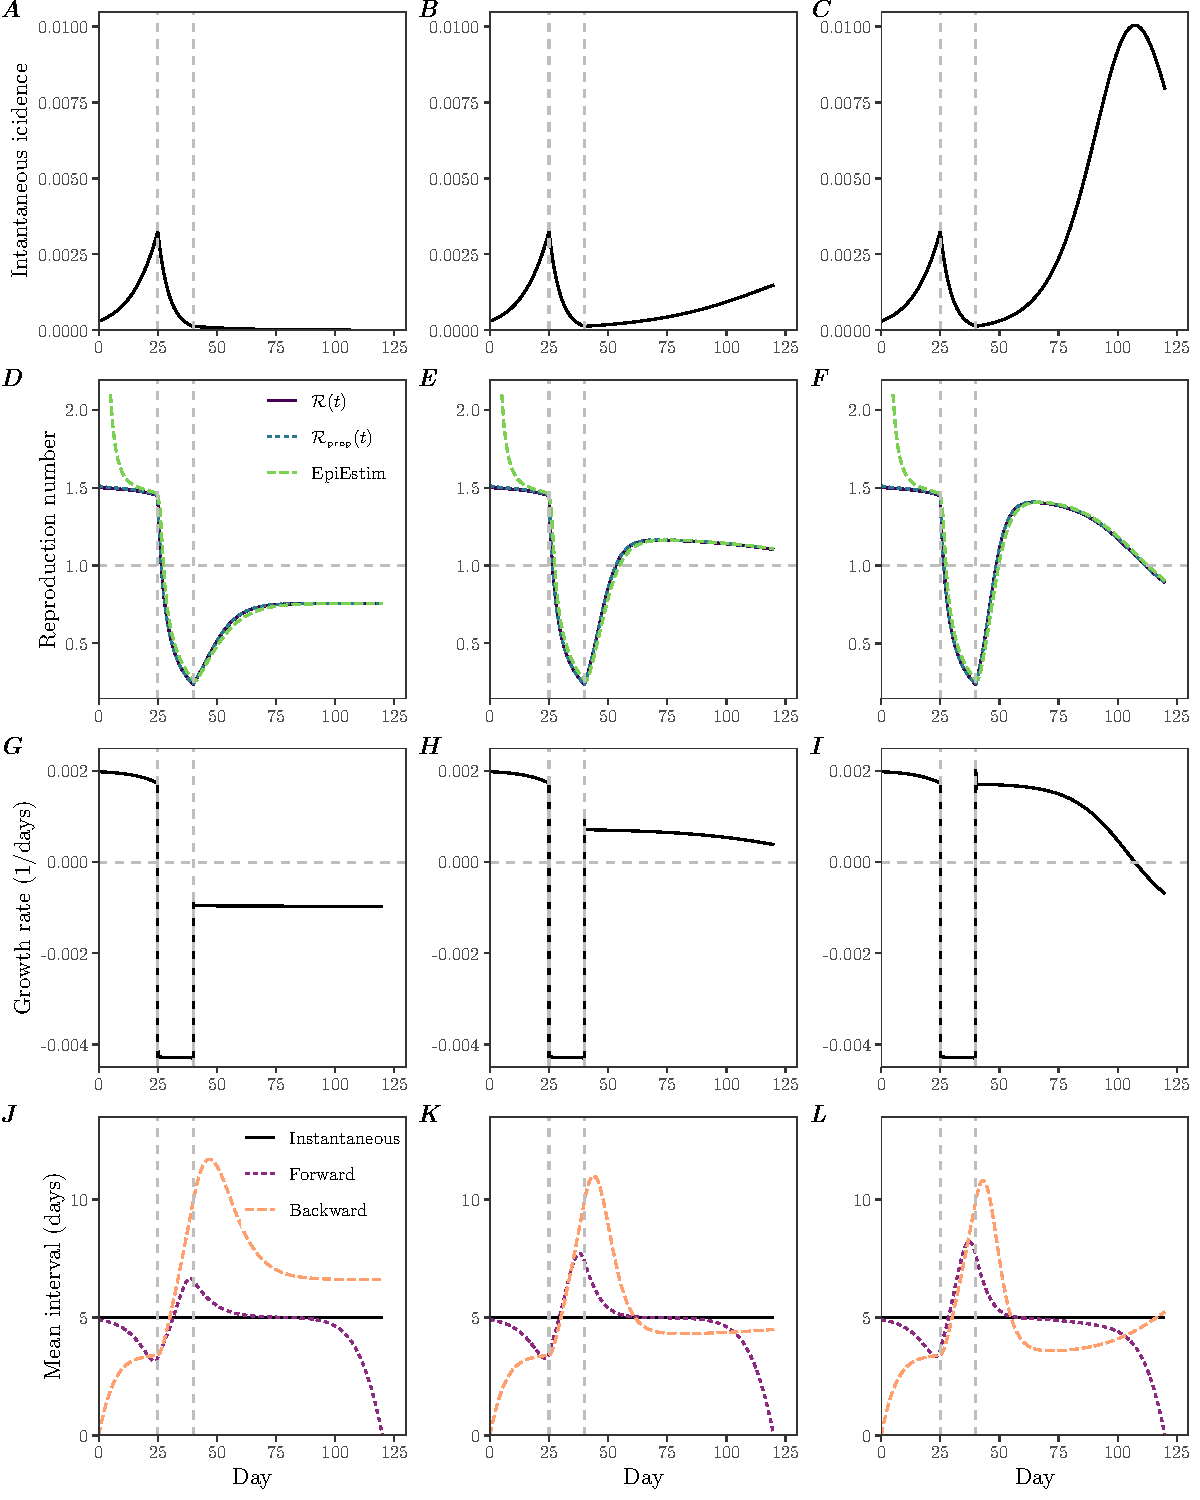
\includegraphics[width=\textwidth]{figure_sir_beta.pdf}
\caption{
\textbf{Epidemiological dynamics of a semi-mechanistic SIR model under equivalent strength-like intervention.}
(A) Changes in true instantaneous reproduction number $\Ri(t)$, proportional reproduction number $\tsub{\RR}{prop}(t)$, estimated $\Ri(t)$ using EpiEstim, and estimated $\tsub{\RR}{forward}(t)$ using the forward generation-interval distribution.
(B) Changes in true case reproduction number $\Rc(t)$, estimated $\Rc(t)$ using Wallinga-Teunis estimator with intrinsic generation-interval distribution, and estimated $\tsub{\RR}{forward}(t)$ using the forward generation-interval distribution.
(C) Changes in mean instantaneous, forward, and backward generation intervals.
}
\label{fig:sir_beta}
\end{figure}

Epidemiological dynamics under equivalent strength-like interventions are presented in \fref{sir_beta}.
In this case, the proportional reproduction number $\tsub{\RR}{prop}(t)$, which relies on the intrinsic generation-interval distribution, matches the instantaneous reproduction number $\Ri(t)$, which relies on the instantaneous generation-interval distribution (\fref{sir_beta}A).
Therefore, we are able to correctly estimate $\Ri(t)$ using \texttt{EpiEstim} (\fref{sir_beta}A)---
minor differences between \texttt{EpiEstim} estimates and $\tsub{\RR}{prop}(t)$ are caused by discretization.

Likewise, we can accurately estimates the case reproduction number $\Rc(t)$ using the Wallinga-Teunis estimator based the intrinsic generation-interval distribution (\fref{sir_beta}B).
This is because the instantaneous generation-interval distribution does not change over time under strength-like interventions (\fref{sir_beta}C).
Using the forward generation-interval distribution, instead of the instantaneous generation-interval distribution, yields smooth, biased estimates of $\Ri(t)$ ($\tsub{\RR}{forward}(t)$ in \fref{sir_beta}A) because the forward distribution changes, even when the instantaneous distribution does not change (\fref{sir_beta}C);
instead, its shape better matches that of $\Rc(t)$.
As described earlier (\fref{indpop}A--C), introducing and lifting strength-like interventions cause the forward generation intervals become shorter and longer, respectively (\fref{sir_beta}C);
the backward distribution exaggerates these changes as it depends on the forward distributions as well as previous incidence.

Epidemiological dynamics under equivalent speed-like interventions are presented in \fref{sir_semi}.
In this case, $\tsub{\RR}{prop}(t)$ differs from the true $\Ri(t)$ (\fref{sir_semi}A) because changes in the instantaneous generation-interval distribution, caused by speed-like interventions (\fref{sir_semi}C).
Therefore, \texttt{EpiEstim} inaccurately estimates $\Ri(t)$ (\fref{sir_semi}A)---
in particular, \texttt{EpiEstim} estimates that $\Ri(t)$ crossed the threshold $\Ri(t)=1$ much later (around $t=60$) than it actually did (around $t=45$).

Using the intrinsic distribution is also problematic for estimating the case reproduction number $\Rc(t)$ (\fref{sir_semi}B).
The true $\Rc(t)$ changes sharply, reflecting sharp changes in the removal rate $\gamma(t)$ (\fref{assumption}B), but using the intrinsic distribution gives smooth estimates of $\Rc(t)$.
In addition, $\tsub{\RR}{forward}(t)$ matches $\Ri(t)$ and $\Rc(t)$ better than their corresponding estimates using the intrinsic generation-interval distribution (EpiEstim and Wallinga-Teunis in \fref{sir_semi}, respectively) because the forward generation-interval distribution captures the effects of speed-like interventions (\fref{sir_semi}C).
Surprisingly, the backward generation-interval distribution stays nearly constant because the effect of decreasing incidence (which lengthens the backward generation intervals) cancels out with that of shorter realized generation intervals, caused by speed-like interventions (\fref{sir_semi}C).

Under both equivalent strength- and speed-like intervention scenarios, we see that neither $\Ri(t) > 1$ nor $\Rc(t) > 1$ necessarily correspond to increasing incidence, $r(t) > 0$ (compare \fref{assumption}D with \fref{sir_beta} and \fref{sir_semi}).
That is, incidence of infection $i(t)$ can increase (or decrease) at any given time $t$ even when $\Ri(t) < 1$ or $\Rc(t) < 1$ (and $\Ri(t) > 1$ or $\Rc(t) > 1$).
Since $\Ri(t)$ is a counterfactual quantity, it does not describe what is happening at time $t$; instead it describes what can happen after time $t$ if conditions remain unchanged.
Since $\Rc(t)$ describes what happened after time $t$, it is also not a good measure for what is happening at time $t$.
On the other hand, $r(t)$ describes what is happening at time $t$ by definition.

\begin{figure}
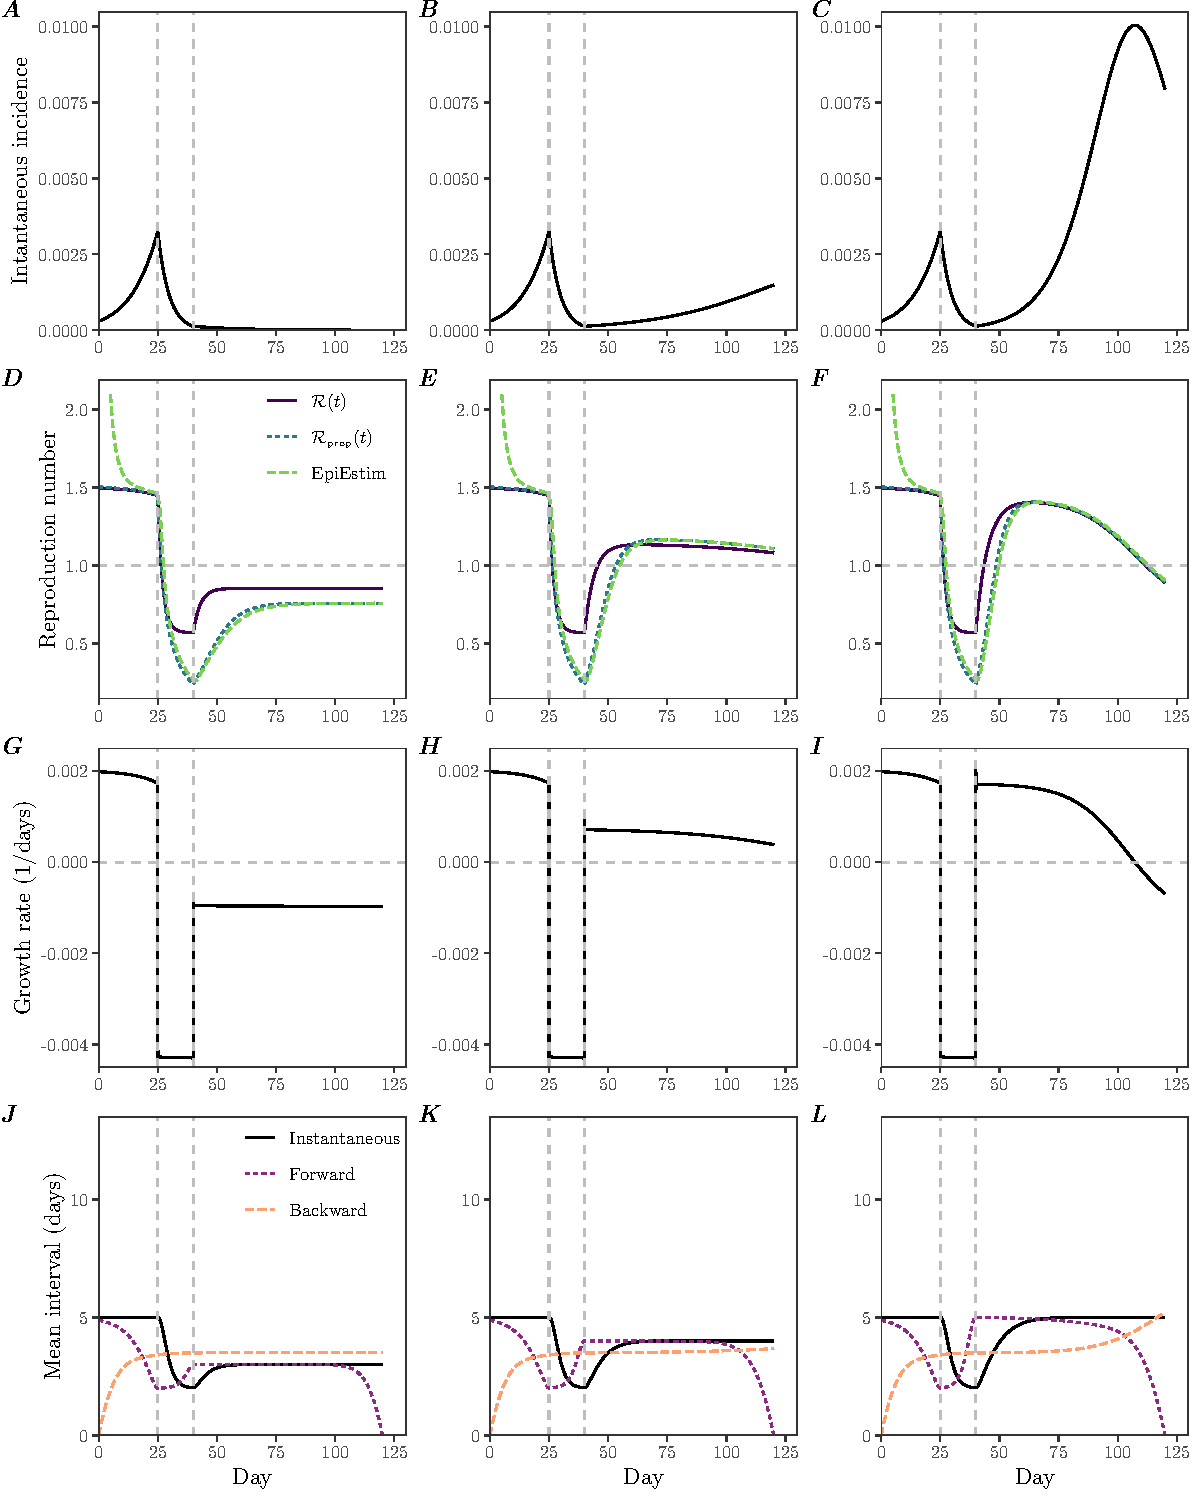
\includegraphics[width=\textwidth]{figure_sir_semi.pdf}
\caption{
\textbf{Epidemiological dynamics of a semi-mechanistic SIR model under equivalent speed-like intervention.}
(A) Changes in true instantaneous reproduction number $\Ri(t)$, proportional reproduction number $\tsub{\RR}{prop}(t)$, estimated $\Ri(t)$ using EpiEstim, and estimated $\tsub{\RR}{forward}(t)$ using the forward generation-interval distribution.
(B) Changes in true case reproduction number $\Rc(t)$, estimated $\Rc(t)$ using Wallinga-Teunis estimator with intrinsic generation-interval distribution, and estimated $\tsub{\RR}{forward}(t)$ using the forward generation-interval distribution.
(C) Changes in mean instantaneous, forward, and backward generation intervals.
}
\label{fig:sir_semi}
\end{figure}

\section{Discussion}

The impact of epidemic interventions are often characterized by changes in ``effective'' reproduction numbers, $\RR(t)$.
Despite historical emphasis on estimating $\RR(t)$, current frameworks neglect possibility that the underlying generation-interval distribution can change over time---an insight that goes back $>10$ years \citep{fraser2007estimating}.
Here, we distinguish two reproduction numbers: instantaneous reproduction number $\Ri(t)$ and case reproduction number $\Rc(t)$, describing counterfactual and realized transmission processes, respectively.
We then show a counterfactual generation-interval distribution, which we refer to as the instantaneous generation-interval distribution, is required to correctly estimate the instantaneous reproduction number. 
This distribution is affected by speed-like, but not strength-like, interventions.
Neglecting changes in this distribution biases estimates of $\Ri(t)$, including when $\Ri(t)$ crosses the threshold value of 1.





\section{Methods}


Here, we consider a simple scenario in which a flu-like pathogen with $\Ro = 1.5$ invades an immunologically naive population.
In the beginning, the disease spreads without any intervention.
On day 25, an intense case isolation measure is implemented. 
On day 40, the intervention is completely/partially lifted.
This is modeled as follows:
\begin{equation}
\beta(t) = 3/10\,\,\textrm{days}^{-1}, \gamma(t) = \begin{cases}
1/5\,\, \textrm{days}^{-1} & t < 25\\
1/2\,\, \textrm{days}^{-1} & 25 \leq t < 40 \\
\tsub{\gamma}{late} & 40 \leq t
\end{cases},
\end{equation}
where we vary $\tsub{\gamma}{late}$ between $1/3\,\, \textrm{days}^{-1}$ (partial lifting) and $1/5\,\, \textrm{days}^{-1}$ (complete lifting).
Simulations are run for 100 days based on the following initial conditions: $S(0) = 1 - 10^{-3}$, $I(0) = 10^{-3}$, and $R(0) = 0$.

Since we assume that incidence is known exactly until time $t^\ast$, we can, in fact, estimate the transmission rate $\beta^\ast(t)$ (with fixed $\gamma(t)=\gamma(0)$) that gives identical incidence trajectory until time $t^\ast$.
This transmission rate is given by:
\begin{equation}
\beta^\ast(t) = \frac{\tsub{\RR}{prop}(t)\gamma(0)}{S(t)}.
\end{equation}
More generally, given true incidence $i(t)$ and true $\RR(t)$ until time $t^\ast$, modulated by some combination of population- and individual-based intervention, we can find population intervention $\PP^\ast(t)$ that gives identical incidence until time $t^\ast$:
\begin{equation}
\PP^\ast(t) = \frac{\tsub{\RR}{prop}(t)}{S(t)}.
\end{equation}
We refer to this intervention as the \emph{equivalent} population-based intervention.

\bibliography{individual_intervention}

\end{document}
